
\documentclass{article}
\usepackage[spanish]{babel}
\usepackage[utf8]{inputenc}
\usepackage{amssymb, amsmath, amsbsy, wasysym}
\usepackage{multirow}
\usepackage{graphicx}
\usepackage{hyperref}
\title{Práctica 7\\Redes de computadoras}
\author{Emmanuel Peto Gutiérrez}
\begin{document}
\maketitle

\section{Pasos para desarrollar la práctica}

Se borra la configuración RIP de los routers UNAM, Google y Telmex. Para eso se usa el comando \texttt{no router rip}.

\begin{center}
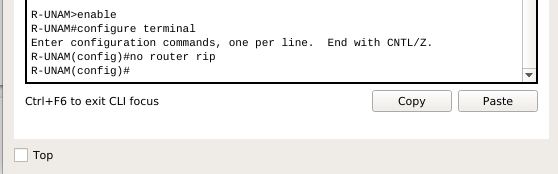
\includegraphics[scale=0.3]{imagenes/1}

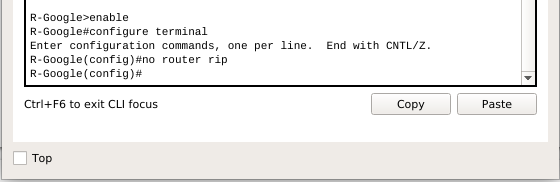
\includegraphics[scale=0.3]{imagenes/2}

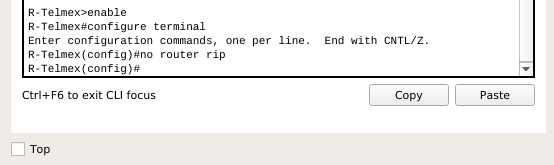
\includegraphics[scale=0.3]{imagenes/3}
\end{center}

En el router de la UNAM se configuran los protocolos RIP y OSPF.

\begin{center}
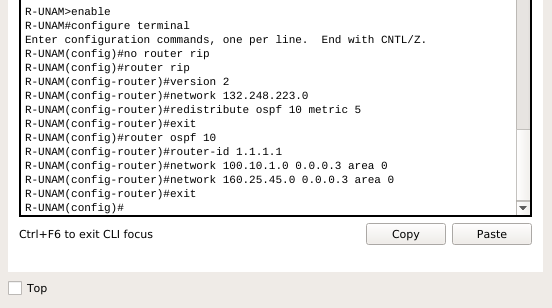
\includegraphics[scale=0.3]{imagenes/4}
\end{center}

En los routers de Google y Telmex se configura solo el protocolo OSPF.

\begin{center}
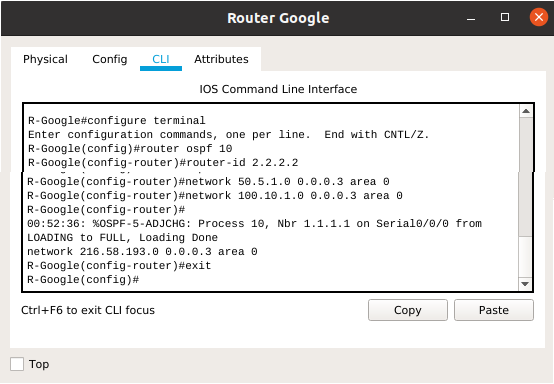
\includegraphics[scale=0.3]{imagenes/5}

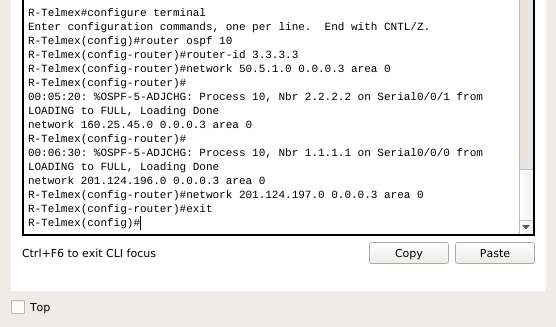
\includegraphics[scale=0.3]{imagenes/6}
\end{center}

Se redistribuyen las rutas entre los routers DGTIC, Ciencias y el SW-Core que utilizan RIP. Esto se hace en el router UNAM.

\begin{center}
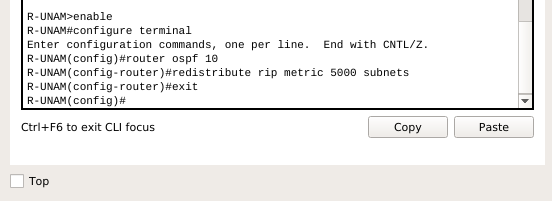
\includegraphics[scale=0.3]{imagenes/7}
\end{center}

Se guarda la configuración de cada router con \texttt{copy running-config startup-config}.

Para ver la configuración de cada router se ejecutan los siguientes comandos:\\
\texttt{show ip interface brief}\\
\texttt{show ip route rip}\\
\texttt{show ip route ospf}\\
\texttt{show ip route}

En los routers de Google y Telmex, el comando \texttt{show ip route rip} no muestra nada porque está inactivo este protocolo.

\begin{center}
UNAM

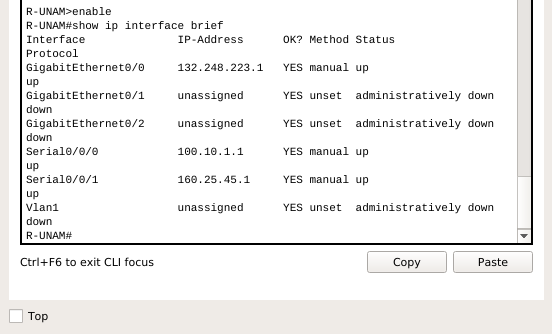
\includegraphics[scale=0.3]{imagenes/8}

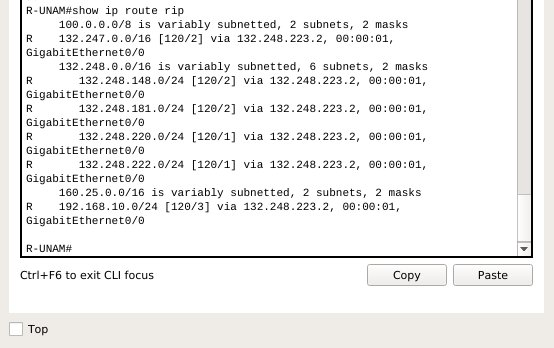
\includegraphics[scale=0.3]{imagenes/9}

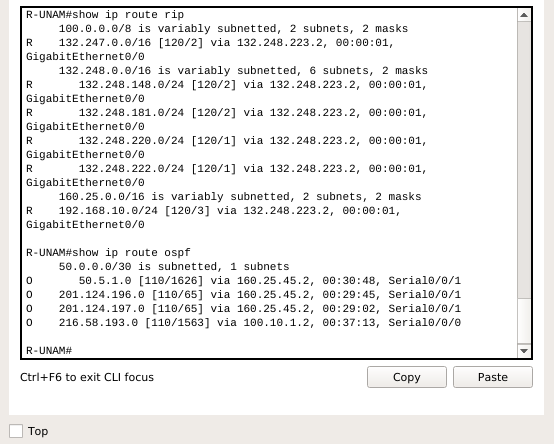
\includegraphics[scale=0.3]{imagenes/10}

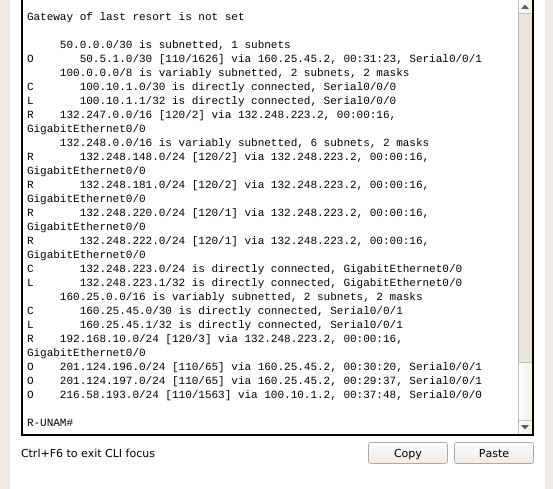
\includegraphics[scale=0.3]{imagenes/11}

Google

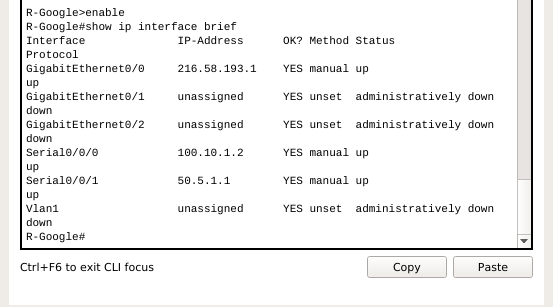
\includegraphics[scale=0.3]{imagenes/12}

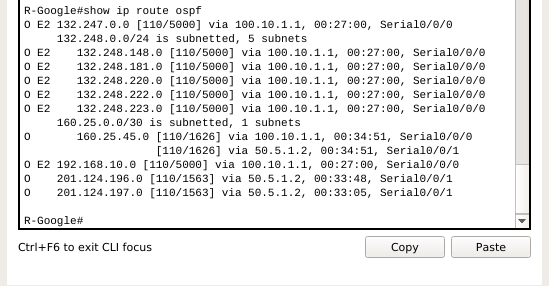
\includegraphics[scale=0.3]{imagenes/13}

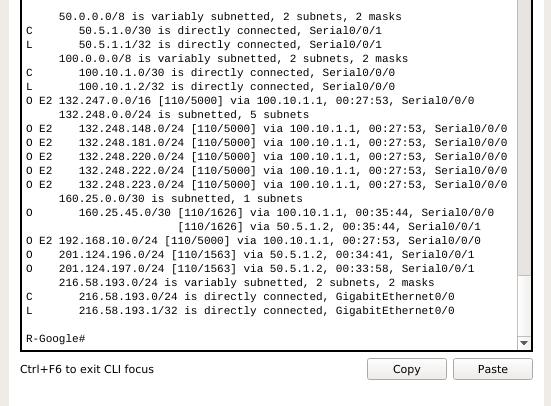
\includegraphics[scale=0.3]{imagenes/14}

Telmex

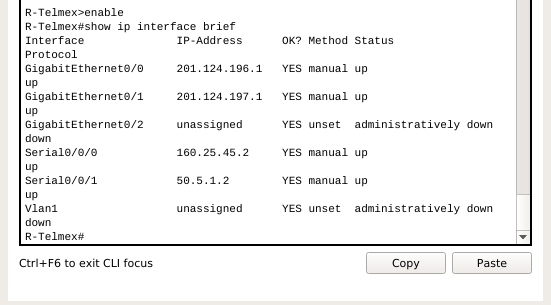
\includegraphics[scale=0.3]{imagenes/15}

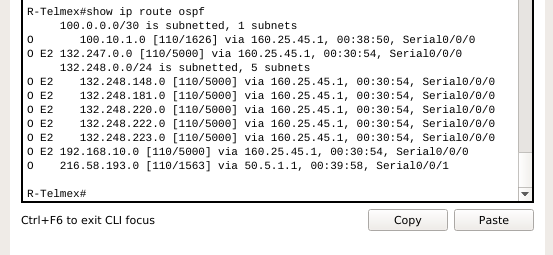
\includegraphics[scale=0.3]{imagenes/16}

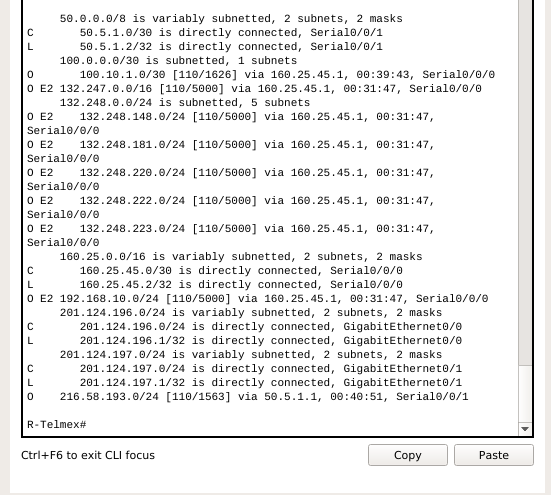
\includegraphics[scale=0.3]{imagenes/17}

\end{center}

Se comprueba que los siguientes dispositivos puedan ingresar a las páginas.

\begin{center}
\begin{tabular}{|c|c|}
\hline
\textbf{Dispositivo} & \textbf{Sitio web} \\ \hline
PC1-DGTIC & www.google.com.mx \\ \hline
A-PC2 & www.google.com.mx \\ \hline
\multirow{2}{*}{Laptop1} & www.unam.mx \\
& www.fciencias.unam.mx\\ \hline
\multirow{3}{*}{Smartphone2} & www.google.com.mx \\
& www.unam.mx \\
& www.fciencias.unam.mx \\ \hline
\end{tabular}
\end{center}

\begin{center}
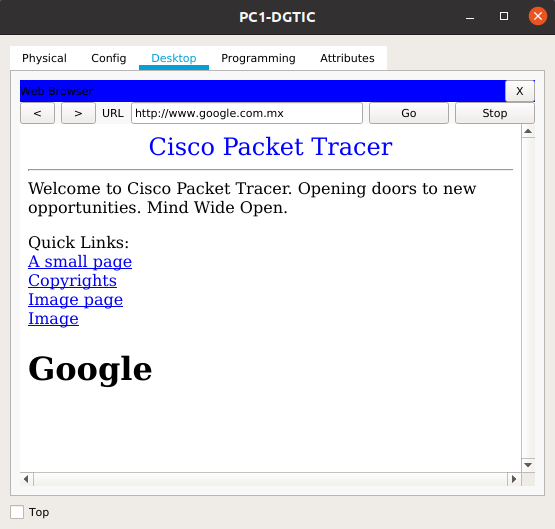
\includegraphics[scale=0.3]{imagenes/18}

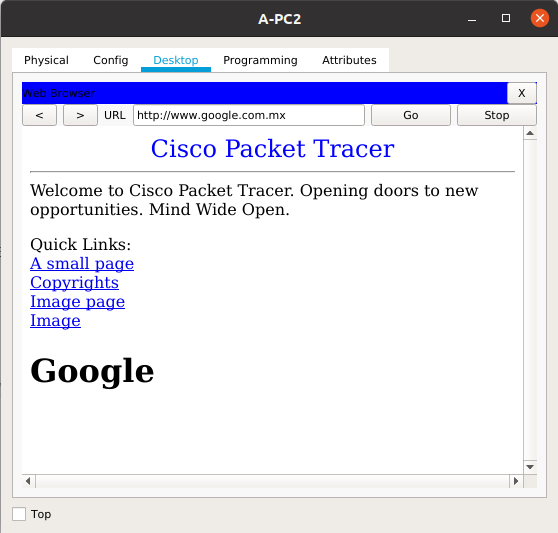
\includegraphics[scale=0.3]{imagenes/19}

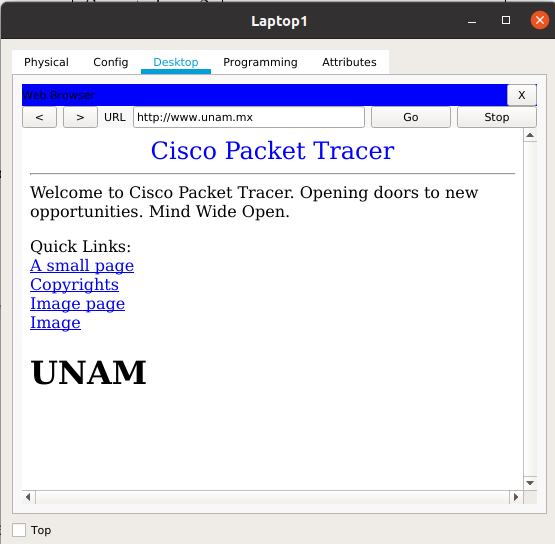
\includegraphics[scale=0.3]{imagenes/20}

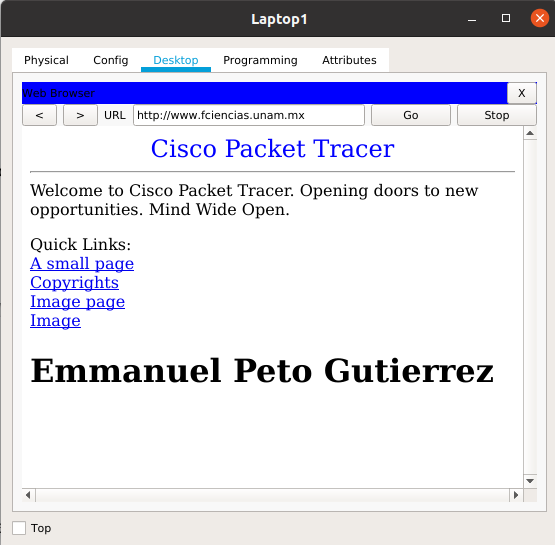
\includegraphics[scale=0.3]{imagenes/21}

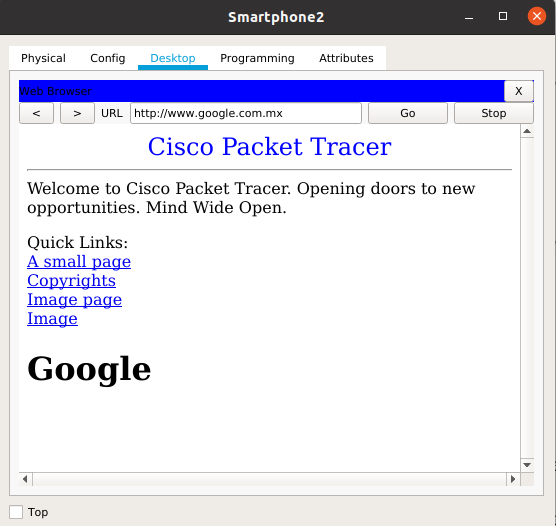
\includegraphics[scale=0.3]{imagenes/22}

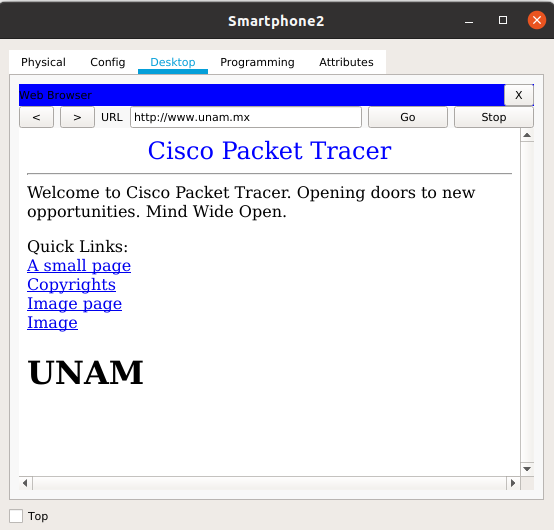
\includegraphics[scale=0.3]{imagenes/23}

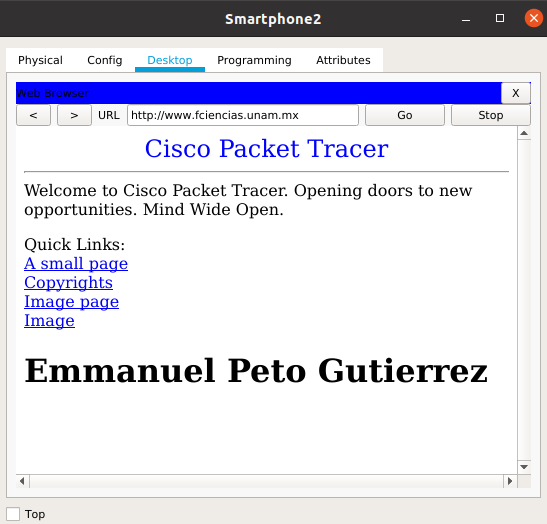
\includegraphics[scale=0.3]{imagenes/24}
\end{center}

Finalmente se muestra la memoria caché de cada servidor DNS.

\begin{center}
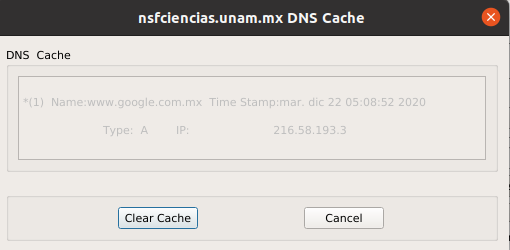
\includegraphics[scale=0.3]{imagenes/25}

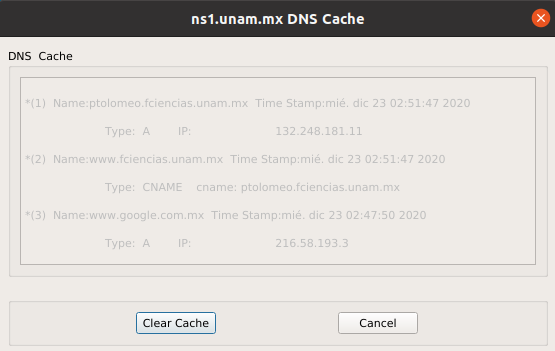
\includegraphics[scale=0.3]{imagenes/26}

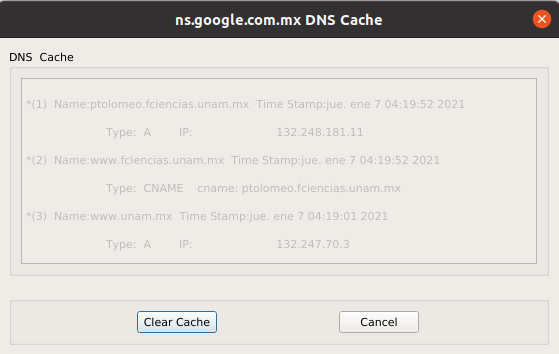
\includegraphics[scale=0.3]{imagenes/27}

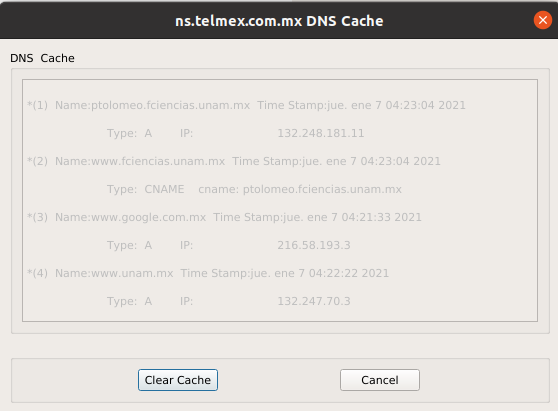
\includegraphics[scale=0.3]{imagenes/28}
\end{center}

\section{Cuestionario}

\begin{itemize}
\item \textbf{¿Qué algoritmo de ruteo implementa OSPF versión 2?}

Es un protocolo link-state que utiliza inundación de información link-state y algoritmo de Dijkstra para calcular la ruta más corta.

\item \textbf{¿Cuáles son las diferencias entre los protocolos de ruteo de interdominio y los protocolos de
ruteo intradominio?}

Los protocolos de ruteo intradominio se ejecutan dentro de un mismo sistema autónomo para determinar la mejor ruta que deben seguir los paquetes, y dentro de un sistema autónomo todos los routers ejecutan el mismo algoritmo.

Un protocolo interdominio se utiliza entre diferentes sistemas autónomos, el cual, para empezar, encuentra el gateway adecuado para que los paquetes salgan del SA. Después, un router del otro lado del SA se encarga de enrutar los paquetes a su destino.

\item \textbf{¿Qué tipo de protocolo de ruteo, interdominio o intradominio, son RIP y OSPF?}

Ambos son intradominio.

\end{itemize}

\end{document}

